\section{Échantillonnage} % (fold)
\label{sec:échantillonnage}

	Nous échantillonons des souches de \esp{Wolbachia} appartenant à des groupes intra-spécifiques identiques sur la base du gène-marqueur \textit{wsp}, un gène dont la variabiité est suffisante pour distinguer des groupes à l'échelle intra-spécifique. Ces groupes sont nommés en général en fonction de leur hôte (\esp{wMel} est la bactérie infectant la drosophile \esp{Drosophila melanogaster} par exemple).

	Notons parmi ces souches que l'on peut ensuite les regrouper dans des groupes encore plus homogènes, car contenant des bactéries identiques sur la base de la concaténation de plusieurs séquences hautement variables à la manière de \textit{wsp}.
	C'est le cas par exemple de \esp{wRi} et de \esp{wAur}, qui formeront un groupe que nous appellerons \esp{wRi-like}.
	\begin{figure}[h]
		\begin{center}
		\begin{tabular}{|c|c|c|}
			\hline
			\textbf{Hôte (souche)}			&\textbf{Déjà testées}				&\textbf{Nouvelles}\\
			\hline
			\esp{D. simulans} (wRi)	&Japon (Tokyo)				&Botswana\\
									&France (Grand Ferrade)		&Afrique du Sud\\
									&Portugal (Chicharo)		& \\
									&Mozambique (Chimoio)		& \\
			\hline
			\esp{D. melanogaster} (wMel)& USA (Seattle) 		& Botswanna (4 sites)\\
									&Pérou						&Zimbabwe\\
									&Madagascar					& \\
			\hline
			\esp{D. auraria} (wAur)	& Terrain (1 échantillon)	&Japon\\
			\hline
			\esp{D. triauraria} (wTriaur)&							&Japon\\
			\hline
			\esp{D. suzukii} (wSuz)	&							&France(6 sites)\\
									& 							&Japon\\
			\hline
			\esp{D. subpulchrella} (wSub)		&							&Japon\\
			\hline
		\end{tabular}
		\end{center}
		\caption{Tableau récapitulatif de la répartition spatiale des échantillons de drosophiles, ainsi que du nom de leurs \esp{Wolbachia} associées. 62 échantillons au total. La colonne «déjà testées» liste la répartition des échantillons ayant déjà été testés lors des traveaux de Hélène \textsc{Henri}\cite{memHH}, avec l'ancienne version du protocole (Cf. partie \ref{sec:transposon_display}), et la colonne «nouvelle» correspond aux nouvelles lignées testées lors de ce stage, avec la nouvelle version du protocole.}
		\label{fig:tab1}
	\end{figure}

	L'échantillonnage a été réalisé sur de multiples souches, issues de lignées de drosophiles provenant de plusieurs origines géographiques (voir tableau \ref{fig:tab1}), afin d'avoir une vue de la variabilité de notre marqueur tant sur une distrubution basée sur la phylogénie de l'hôte que sur un plan spatial.

	% \paragraph{\textit{L. heterotoma}} % (fold)
	% \label{par:hetero_mm}
	% \textit{L. heterotoma} étant dans la nature infectées par trois souches distinctes de \esp{Wolbachia}, il faut, pour typer celles-ci en Transposon-display, obtenir des lignées mono-infectées. Pour cela, nous appliquons une méthode basée sur des traitements antibiotiques ménagés, que nous décrivons en annexe, non décrits dans ce rapport.
	% % paragraph hetero_mm (end)

% subsection échantillonnage (end)

\section{Extractions d'ADN et statuts d'infection} % (fold)
L'ADN génomique des échantillons de drosophiles a été extrait au moyen du kit d'extraction \textit{NucleoSpin® Tissue}, de l'entreprise Macherey-Nagel.
Ce kit nous permet d'avoir un ADN purifié, certaines étapes de la technique du transposon-display étant très sensibles aux divers inhibiteurs que l'on pourrait trouver dans des échantillons extraits avec des protocoles plus simples.

L'efficacité des extractions a été vérifié par PCR sur la base du gène mitochondrial \textit{Its2}, gène très généraliste. Pour cette PCR, un extrait issu d'une extraction antérieure a été pris comme témoin positif.

Les statuts d'infection ont été déterminés sur la base du gène \textit{Fts-Z}, spécifique de \esp{Wolbachia}. Nous avons pris un extrait issu d'une autre extraction, dont le statut d'infection était connu comme étant positif comme témoin positif, et un extrait d'une drosophile traitée par antibiotique, vérifiée comme étant exempte de \esp{Wolbachia} comme témoin négatif.

Pour les échantillons positifs sur \textit{Fts-Z} (donc inféctés par Wolbachia), nous avons effectué un séquencage du gène \textit{wsp} afin de déterminer la souche de \esp{Wolbachia}.

% Parler de COI ssi y'a assez de place.

Enfin, la présence du transposon \textit{ISWpi1}, utilisé pour le transposon-display, a été vérifié par PCR avec les amorces ISWpi1-F/ISWpi1-R.

\section{Transposon-display} % (fold)
\label{sec:transposon_display}

	\paragraph{Principe général} % (fold)
	\label{par:principe_TnDisp}
	Le transposon-display est une méthode de biologie moléculaire visant à établir un \textit{fingerprint} des locus d'insertion d'un transposon. 
	Elle est tirée de la méthode ASAP (Allele-Specific Alu PCR)\cite{ASAP}, et adapté au contexte \esp{Wolbachia}/\textit{ISWpi1} par Hélène \textsc{Henri}\cite{memHH}.\\
	Nous allons décrire ici brièvement son principe (voir le schéma \ref{fig:figure1})~:
	\begin{enumerate}
		\item Le génome est digéré par une enzyme de restriction (ici, HindIII), séléctionné pour couper de façon fréquente le génome, mais n'ayant pas son motif de coupure dans le transposon.
		\item Des adaptateurs
		%\footnote{Dessinés par Hélène \textsc{Henri}, décrits dans son mémoire \cite{memHH}}
		% Je pense qu'on aura compris ^^
		sont ensuite appliqués à cet ADN digéré, conçus pour être d'un côté complémentaires au motif de coupure de HindIII, et de l'autre pour ne pas être complémentaire sur la fin, afin de former un "Y" qui permettra d'éviter les amplifications non-spécifiques pour les fragments de petite taille.
		%\item Nous nous retrouvons donc avec une série de fragments linéaires d'ADN de l'échantillon, flanqués de notre adaptateur, contenant pour certains le transposon qui nous intéresse (\textit{ISWpi2}).
		% Ça c'est du langage oral, c'est déplacé.
		\item L'étape finale consiste en deux PCR, avec comme amorce commune une amorce spécifique à l'adaptateur (La partie en "Y"), et l'autre soit à la partie 5' du transposon (ISb), soit la partie 3' (ISc).
	\end{enumerate}
	% Le résultat (renvoyer à figure gels) de cette PCR, après éléctrophorèse, nous donne un \textit{barcode} dans lequel chaque bande correspond à un locus d'insertion du transposon.
	Après migration sur gel d'éléctrophorèse, nous obtenons un profil dans lequel chaque fragment correspond à un locus d'insertion du transposon.
	% paragraph principe_TnDisp (end)

	\paragraph{Des nouveautés dans le protocole} % (fold)
	\label{par:protocole2}
	Ce stage a été l'occasion pour tester une amélioration du protocole du transposon-display, en particulier au niveau de la PCR, avec l'utilisation d'une Taq-polymérase haute fidélité (AccuTaq de la société Sigma), et l'ajustement en conséquence du programme de thermocycleur.
	% paragraph protocole2 (end)

\begin{figure}[h!]
	\begin{center}
		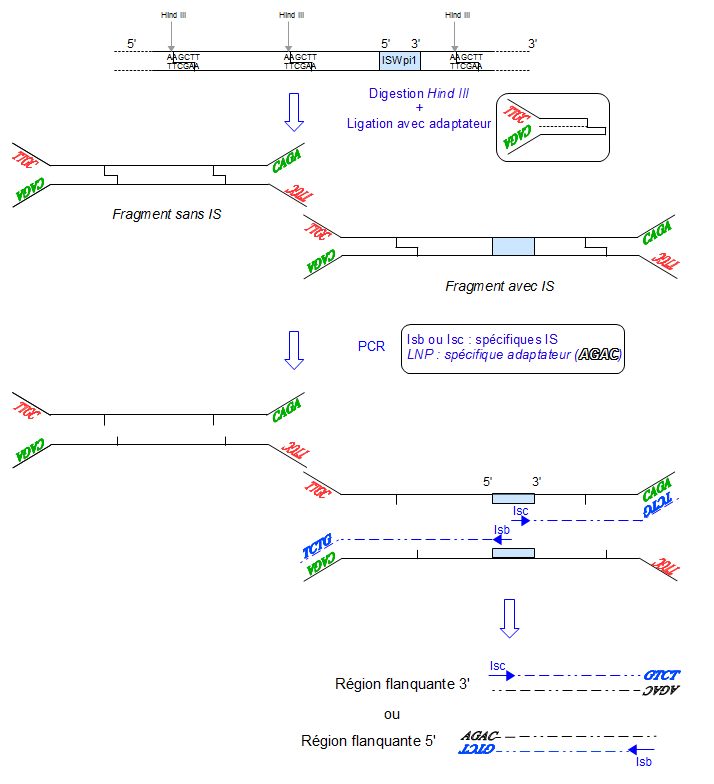
\includegraphics[width=160mm]{tdisplay.png}
	\end{center}
	\caption{Principe du Transposon Display avec amplification sélective des régions
flanquantes des insertions. Figure povenant du mémoire de Hélène \textsc{Henri}\cite{memHH}.% Là j'aimerais bien footciter, mais y'a un bug connu quand on footnote des trucs depuis une caption :(
	}
	\label{fig:figure1}
\end{figure}

% subsection transposon_display (end)
